% Graphic for TeX using PGF
% Title: /home/alex/Documents/Schule/Diplomarbeit/diplatex/dia/model.dia
% Creator: Dia v0.97
% CreationDate: Mon May 17 13:13:05 2010
% For: alex
% \usepackage{tikz}
% The following commands are not supported in PSTricks at present
% We define them conditionally, so when they are implemented,
% this pgf file will use them.
\ifx\du\undefined
  \newlength{\du}
\fi
\setlength{\du}{15\unitlength}
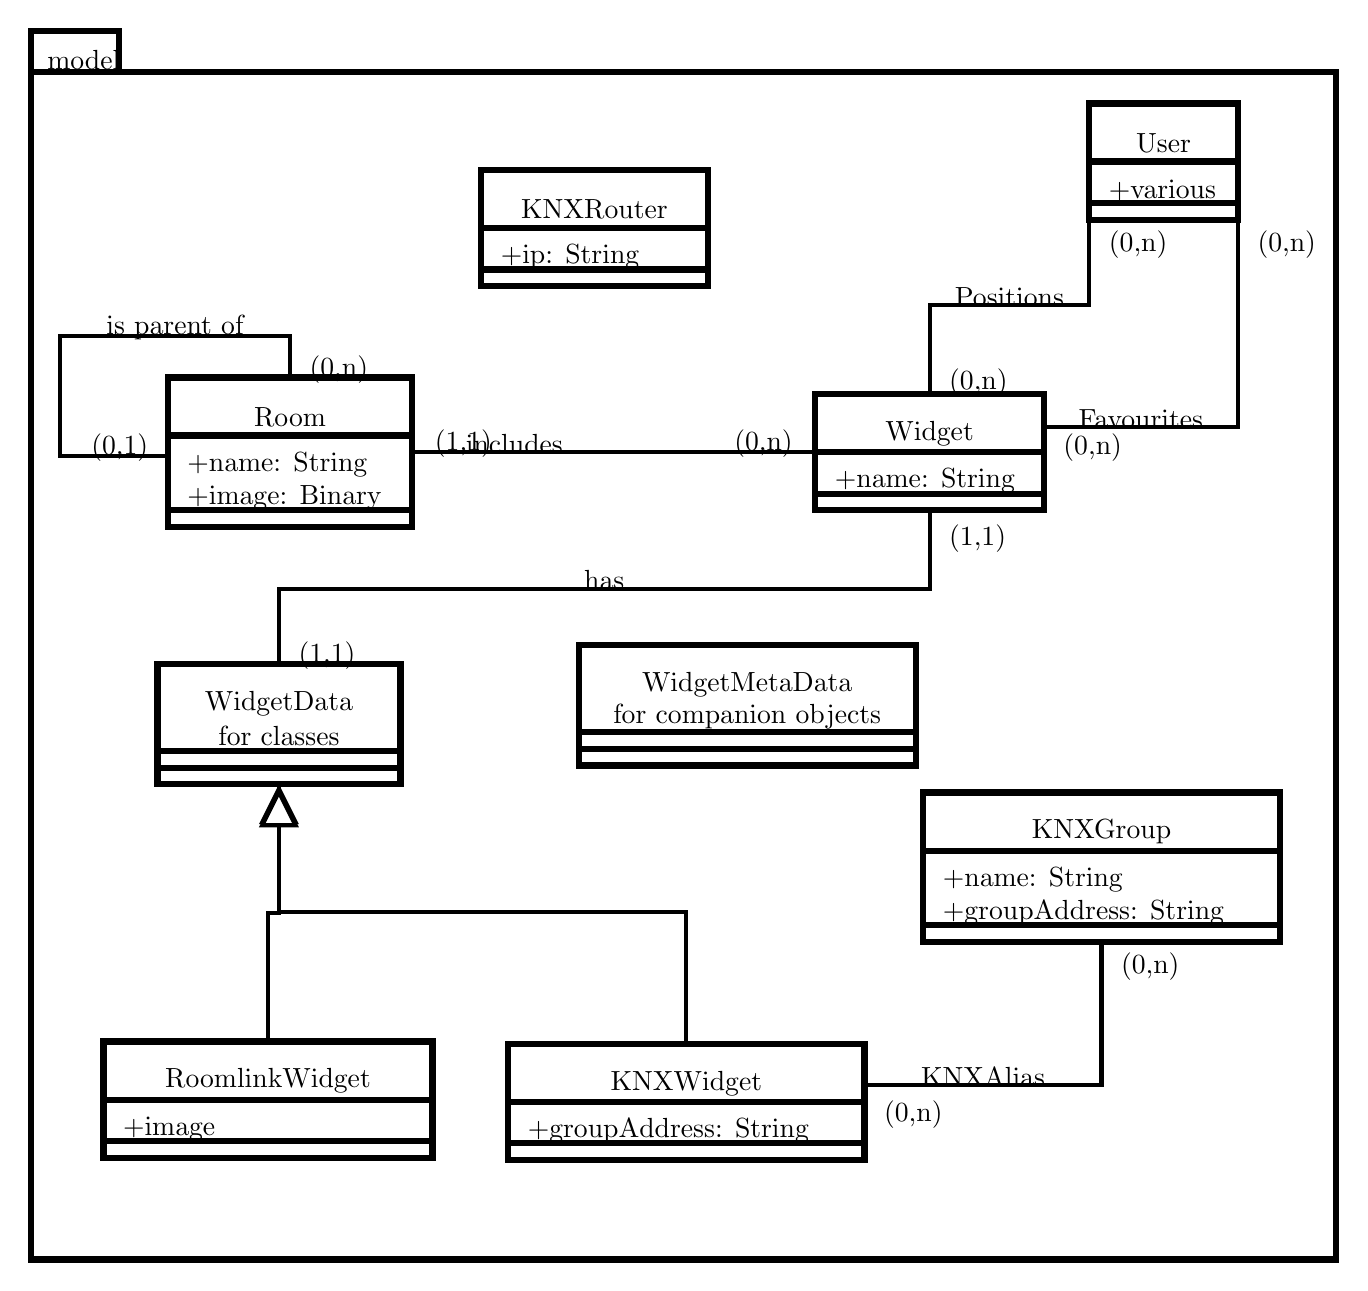
\begin{tikzpicture}
\pgftransformxscale{1.000000}
\pgftransformyscale{-1.000000}
\definecolor{dialinecolor}{rgb}{0.000000, 0.000000, 0.000000}
\pgfsetstrokecolor{dialinecolor}
\definecolor{dialinecolor}{rgb}{1.000000, 1.000000, 1.000000}
\pgfsetfillcolor{dialinecolor}
\pgfsetlinewidth{0.150000\du}
\pgfsetdash{}{0pt}
\definecolor{dialinecolor}{rgb}{1.000000, 1.000000, 1.000000}
\pgfsetfillcolor{dialinecolor}
\fill (15.300000\du,1.300000\du)--(15.300000\du,29.900000\du)--(46.750000\du,29.900000\du)--(46.750000\du,1.300000\du)--cycle;
\definecolor{dialinecolor}{rgb}{0.000000, 0.000000, 0.000000}
\pgfsetstrokecolor{dialinecolor}
\draw (15.300000\du,1.300000\du)--(15.300000\du,29.900000\du)--(46.750000\du,29.900000\du)--(46.750000\du,1.300000\du)--cycle;
\definecolor{dialinecolor}{rgb}{1.000000, 1.000000, 1.000000}
\pgfsetfillcolor{dialinecolor}
\fill (15.300000\du,0.300000\du)--(15.300000\du,1.300000\du)--(17.425000\du,1.300000\du)--(17.425000\du,0.300000\du)--cycle;
\definecolor{dialinecolor}{rgb}{0.000000, 0.000000, 0.000000}
\pgfsetstrokecolor{dialinecolor}
\draw (15.300000\du,0.300000\du)--(15.300000\du,1.300000\du)--(17.425000\du,1.300000\du)--(17.425000\du,0.300000\du)--cycle;
% setfont left to latex
\definecolor{dialinecolor}{rgb}{0.000000, 0.000000, 0.000000}
\pgfsetstrokecolor{dialinecolor}
\node[anchor=west] at (15.400000\du,1.000000\du){model};
\pgfsetlinewidth{0.150000\du}
\pgfsetdash{}{0pt}
\definecolor{dialinecolor}{rgb}{1.000000, 1.000000, 1.000000}
\pgfsetfillcolor{dialinecolor}
\fill (18.600000\du,8.650000\du)--(18.600000\du,10.050000\du)--(24.490000\du,10.050000\du)--(24.490000\du,8.650000\du)--cycle;
\definecolor{dialinecolor}{rgb}{0.000000, 0.000000, 0.000000}
\pgfsetstrokecolor{dialinecolor}
\draw (18.600000\du,8.650000\du)--(18.600000\du,10.050000\du)--(24.490000\du,10.050000\du)--(24.490000\du,8.650000\du)--cycle;
% setfont left to latex
\definecolor{dialinecolor}{rgb}{0.000000, 0.000000, 0.000000}
\pgfsetstrokecolor{dialinecolor}
\node at (21.545000\du,9.600000\du){Room};
\definecolor{dialinecolor}{rgb}{1.000000, 1.000000, 1.000000}
\pgfsetfillcolor{dialinecolor}
\fill (18.600000\du,10.050000\du)--(18.600000\du,11.850000\du)--(24.490000\du,11.850000\du)--(24.490000\du,10.050000\du)--cycle;
\definecolor{dialinecolor}{rgb}{0.000000, 0.000000, 0.000000}
\pgfsetstrokecolor{dialinecolor}
\draw (18.600000\du,10.050000\du)--(18.600000\du,11.850000\du)--(24.490000\du,11.850000\du)--(24.490000\du,10.050000\du)--cycle;
% setfont left to latex
\definecolor{dialinecolor}{rgb}{0.000000, 0.000000, 0.000000}
\pgfsetstrokecolor{dialinecolor}
\node[anchor=west] at (18.775000\du,10.750000\du){+name: String};
% setfont left to latex
\definecolor{dialinecolor}{rgb}{0.000000, 0.000000, 0.000000}
\pgfsetstrokecolor{dialinecolor}
\node[anchor=west] at (18.775000\du,11.550000\du){+image: Binary};
\definecolor{dialinecolor}{rgb}{1.000000, 1.000000, 1.000000}
\pgfsetfillcolor{dialinecolor}
\fill (18.600000\du,11.850000\du)--(18.600000\du,12.250000\du)--(24.490000\du,12.250000\du)--(24.490000\du,11.850000\du)--cycle;
\definecolor{dialinecolor}{rgb}{0.000000, 0.000000, 0.000000}
\pgfsetstrokecolor{dialinecolor}
\draw (18.600000\du,11.850000\du)--(18.600000\du,12.250000\du)--(24.490000\du,12.250000\du)--(24.490000\du,11.850000\du)--cycle;
\pgfsetlinewidth{0.150000\du}
\pgfsetdash{}{0pt}
\definecolor{dialinecolor}{rgb}{1.000000, 1.000000, 1.000000}
\pgfsetfillcolor{dialinecolor}
\fill (34.200000\du,9.050000\du)--(34.200000\du,10.450000\du)--(39.705000\du,10.450000\du)--(39.705000\du,9.050000\du)--cycle;
\definecolor{dialinecolor}{rgb}{0.000000, 0.000000, 0.000000}
\pgfsetstrokecolor{dialinecolor}
\draw (34.200000\du,9.050000\du)--(34.200000\du,10.450000\du)--(39.705000\du,10.450000\du)--(39.705000\du,9.050000\du)--cycle;
% setfont left to latex
\definecolor{dialinecolor}{rgb}{0.000000, 0.000000, 0.000000}
\pgfsetstrokecolor{dialinecolor}
\node at (36.952500\du,10.000000\du){Widget};
\definecolor{dialinecolor}{rgb}{1.000000, 1.000000, 1.000000}
\pgfsetfillcolor{dialinecolor}
\fill (34.200000\du,10.450000\du)--(34.200000\du,11.450000\du)--(39.705000\du,11.450000\du)--(39.705000\du,10.450000\du)--cycle;
\definecolor{dialinecolor}{rgb}{0.000000, 0.000000, 0.000000}
\pgfsetstrokecolor{dialinecolor}
\draw (34.200000\du,10.450000\du)--(34.200000\du,11.450000\du)--(39.705000\du,11.450000\du)--(39.705000\du,10.450000\du)--cycle;
% setfont left to latex
\definecolor{dialinecolor}{rgb}{0.000000, 0.000000, 0.000000}
\pgfsetstrokecolor{dialinecolor}
\node[anchor=west] at (34.375000\du,11.150000\du){+name: String};
\definecolor{dialinecolor}{rgb}{1.000000, 1.000000, 1.000000}
\pgfsetfillcolor{dialinecolor}
\fill (34.200000\du,11.450000\du)--(34.200000\du,11.850000\du)--(39.705000\du,11.850000\du)--(39.705000\du,11.450000\du)--cycle;
\definecolor{dialinecolor}{rgb}{0.000000, 0.000000, 0.000000}
\pgfsetstrokecolor{dialinecolor}
\draw (34.200000\du,11.450000\du)--(34.200000\du,11.850000\du)--(39.705000\du,11.850000\du)--(39.705000\du,11.450000\du)--cycle;
\pgfsetlinewidth{0.150000\du}
\pgfsetdash{}{0pt}
\definecolor{dialinecolor}{rgb}{1.000000, 1.000000, 1.000000}
\pgfsetfillcolor{dialinecolor}
\fill (18.350000\du,15.550000\du)--(18.350000\du,17.650000\du)--(24.205000\du,17.650000\du)--(24.205000\du,15.550000\du)--cycle;
\definecolor{dialinecolor}{rgb}{0.000000, 0.000000, 0.000000}
\pgfsetstrokecolor{dialinecolor}
\draw (18.350000\du,15.550000\du)--(18.350000\du,17.650000\du)--(24.205000\du,17.650000\du)--(24.205000\du,15.550000\du)--cycle;
% setfont left to latex
\definecolor{dialinecolor}{rgb}{0.000000, 0.000000, 0.000000}
\pgfsetstrokecolor{dialinecolor}
\node at (21.277500\du,16.500000\du){WidgetData};
% setfont left to latex
\definecolor{dialinecolor}{rgb}{0.000000, 0.000000, 0.000000}
\pgfsetstrokecolor{dialinecolor}
\node at (21.277500\du,17.275000\du){for classes};
\definecolor{dialinecolor}{rgb}{1.000000, 1.000000, 1.000000}
\pgfsetfillcolor{dialinecolor}
\fill (18.350000\du,17.650000\du)--(18.350000\du,18.050000\du)--(24.205000\du,18.050000\du)--(24.205000\du,17.650000\du)--cycle;
\definecolor{dialinecolor}{rgb}{0.000000, 0.000000, 0.000000}
\pgfsetstrokecolor{dialinecolor}
\draw (18.350000\du,17.650000\du)--(18.350000\du,18.050000\du)--(24.205000\du,18.050000\du)--(24.205000\du,17.650000\du)--cycle;
\definecolor{dialinecolor}{rgb}{1.000000, 1.000000, 1.000000}
\pgfsetfillcolor{dialinecolor}
\fill (18.350000\du,18.050000\du)--(18.350000\du,18.450000\du)--(24.205000\du,18.450000\du)--(24.205000\du,18.050000\du)--cycle;
\definecolor{dialinecolor}{rgb}{0.000000, 0.000000, 0.000000}
\pgfsetstrokecolor{dialinecolor}
\draw (18.350000\du,18.050000\du)--(18.350000\du,18.450000\du)--(24.205000\du,18.450000\du)--(24.205000\du,18.050000\du)--cycle;
\pgfsetlinewidth{0.150000\du}
\pgfsetdash{}{0pt}
\definecolor{dialinecolor}{rgb}{1.000000, 1.000000, 1.000000}
\pgfsetfillcolor{dialinecolor}
\fill (28.500000\du,15.100000\du)--(28.500000\du,17.200000\du)--(36.615000\du,17.200000\du)--(36.615000\du,15.100000\du)--cycle;
\definecolor{dialinecolor}{rgb}{0.000000, 0.000000, 0.000000}
\pgfsetstrokecolor{dialinecolor}
\draw (28.500000\du,15.100000\du)--(28.500000\du,17.200000\du)--(36.615000\du,17.200000\du)--(36.615000\du,15.100000\du)--cycle;
% setfont left to latex
\definecolor{dialinecolor}{rgb}{0.000000, 0.000000, 0.000000}
\pgfsetstrokecolor{dialinecolor}
\node at (32.557500\du,16.050000\du){WidgetMetaData};
% setfont left to latex
\definecolor{dialinecolor}{rgb}{0.000000, 0.000000, 0.000000}
\pgfsetstrokecolor{dialinecolor}
\node at (32.557500\du,16.825000\du){for companion objects};
\definecolor{dialinecolor}{rgb}{1.000000, 1.000000, 1.000000}
\pgfsetfillcolor{dialinecolor}
\fill (28.500000\du,17.200000\du)--(28.500000\du,17.600000\du)--(36.615000\du,17.600000\du)--(36.615000\du,17.200000\du)--cycle;
\definecolor{dialinecolor}{rgb}{0.000000, 0.000000, 0.000000}
\pgfsetstrokecolor{dialinecolor}
\draw (28.500000\du,17.200000\du)--(28.500000\du,17.600000\du)--(36.615000\du,17.600000\du)--(36.615000\du,17.200000\du)--cycle;
\definecolor{dialinecolor}{rgb}{1.000000, 1.000000, 1.000000}
\pgfsetfillcolor{dialinecolor}
\fill (28.500000\du,17.600000\du)--(28.500000\du,18.000000\du)--(36.615000\du,18.000000\du)--(36.615000\du,17.600000\du)--cycle;
\definecolor{dialinecolor}{rgb}{0.000000, 0.000000, 0.000000}
\pgfsetstrokecolor{dialinecolor}
\draw (28.500000\du,17.600000\du)--(28.500000\du,18.000000\du)--(36.615000\du,18.000000\du)--(36.615000\du,17.600000\du)--cycle;
\pgfsetlinewidth{0.100000\du}
\pgfsetdash{}{0pt}
\pgfsetmiterjoin
\pgfsetbuttcap
{
\definecolor{dialinecolor}{rgb}{0.000000, 0.000000, 0.000000}
\pgfsetfillcolor{dialinecolor}
% was here!!!
\definecolor{dialinecolor}{rgb}{0.000000, 0.000000, 0.000000}
\pgfsetstrokecolor{dialinecolor}
\draw (34.127087\du,10.450000\du)--(26.950000\du,10.450000\du)--(26.950000\du,10.450000\du)--(24.564859\du,10.450000\du);
}
% setfont left to latex
\definecolor{dialinecolor}{rgb}{0.000000, 0.000000, 0.000000}
\pgfsetstrokecolor{dialinecolor}
\node at (26.950000\du,10.250000\du){includes};
\definecolor{dialinecolor}{rgb}{0.000000, 0.000000, 0.000000}
\pgfsetstrokecolor{dialinecolor}
\node[anchor=east] at (33.927087\du,10.250000\du){(0,n)};
\definecolor{dialinecolor}{rgb}{0.000000, 0.000000, 0.000000}
\pgfsetstrokecolor{dialinecolor}
\node[anchor=west] at (24.764859\du,10.250000\du){(1,1)};
\pgfsetlinewidth{0.100000\du}
\pgfsetdash{}{0pt}
\pgfsetmiterjoin
\pgfsetbuttcap
{
\definecolor{dialinecolor}{rgb}{0.000000, 0.000000, 0.000000}
\pgfsetfillcolor{dialinecolor}
% was here!!!
\definecolor{dialinecolor}{rgb}{0.000000, 0.000000, 0.000000}
\pgfsetstrokecolor{dialinecolor}
\draw (21.277500\du,15.550000\du)--(21.277500\du,13.737680\du)--(36.952500\du,13.737680\du)--(36.952500\du,11.925360\du);
}
% setfont left to latex
\definecolor{dialinecolor}{rgb}{0.000000, 0.000000, 0.000000}
\pgfsetstrokecolor{dialinecolor}
\node at (29.115000\du,13.537680\du){has};
\definecolor{dialinecolor}{rgb}{0.000000, 0.000000, 0.000000}
\pgfsetstrokecolor{dialinecolor}
\node[anchor=west] at (21.477500\du,15.350000\du){(1,1)};
\definecolor{dialinecolor}{rgb}{0.000000, 0.000000, 0.000000}
\pgfsetstrokecolor{dialinecolor}
\node[anchor=west] at (37.152500\du,12.525360\du){(1,1)};
\pgfsetlinewidth{0.150000\du}
\pgfsetdash{}{0pt}
\definecolor{dialinecolor}{rgb}{1.000000, 1.000000, 1.000000}
\pgfsetfillcolor{dialinecolor}
\fill (26.800000\du,24.700000\du)--(26.800000\du,26.100000\du)--(35.385000\du,26.100000\du)--(35.385000\du,24.700000\du)--cycle;
\definecolor{dialinecolor}{rgb}{0.000000, 0.000000, 0.000000}
\pgfsetstrokecolor{dialinecolor}
\draw (26.800000\du,24.700000\du)--(26.800000\du,26.100000\du)--(35.385000\du,26.100000\du)--(35.385000\du,24.700000\du)--cycle;
% setfont left to latex
\definecolor{dialinecolor}{rgb}{0.000000, 0.000000, 0.000000}
\pgfsetstrokecolor{dialinecolor}
\node at (31.092500\du,25.650000\du){KNXWidget};
\definecolor{dialinecolor}{rgb}{1.000000, 1.000000, 1.000000}
\pgfsetfillcolor{dialinecolor}
\fill (26.800000\du,26.100000\du)--(26.800000\du,27.100000\du)--(35.385000\du,27.100000\du)--(35.385000\du,26.100000\du)--cycle;
\definecolor{dialinecolor}{rgb}{0.000000, 0.000000, 0.000000}
\pgfsetstrokecolor{dialinecolor}
\draw (26.800000\du,26.100000\du)--(26.800000\du,27.100000\du)--(35.385000\du,27.100000\du)--(35.385000\du,26.100000\du)--cycle;
% setfont left to latex
\definecolor{dialinecolor}{rgb}{0.000000, 0.000000, 0.000000}
\pgfsetstrokecolor{dialinecolor}
\node[anchor=west] at (26.975000\du,26.800000\du){+groupAddress: String};
\definecolor{dialinecolor}{rgb}{1.000000, 1.000000, 1.000000}
\pgfsetfillcolor{dialinecolor}
\fill (26.800000\du,27.100000\du)--(26.800000\du,27.500000\du)--(35.385000\du,27.500000\du)--(35.385000\du,27.100000\du)--cycle;
\definecolor{dialinecolor}{rgb}{0.000000, 0.000000, 0.000000}
\pgfsetstrokecolor{dialinecolor}
\draw (26.800000\du,27.100000\du)--(26.800000\du,27.500000\du)--(35.385000\du,27.500000\du)--(35.385000\du,27.100000\du)--cycle;
\pgfsetlinewidth{0.150000\du}
\pgfsetdash{}{0pt}
\definecolor{dialinecolor}{rgb}{1.000000, 1.000000, 1.000000}
\pgfsetfillcolor{dialinecolor}
\fill (17.050000\du,24.650000\du)--(17.050000\du,26.050000\du)--(24.977500\du,26.050000\du)--(24.977500\du,24.650000\du)--cycle;
\definecolor{dialinecolor}{rgb}{0.000000, 0.000000, 0.000000}
\pgfsetstrokecolor{dialinecolor}
\draw (17.050000\du,24.650000\du)--(17.050000\du,26.050000\du)--(24.977500\du,26.050000\du)--(24.977500\du,24.650000\du)--cycle;
% setfont left to latex
\definecolor{dialinecolor}{rgb}{0.000000, 0.000000, 0.000000}
\pgfsetstrokecolor{dialinecolor}
\node at (21.013750\du,25.600000\du){RoomlinkWidget};
\definecolor{dialinecolor}{rgb}{1.000000, 1.000000, 1.000000}
\pgfsetfillcolor{dialinecolor}
\fill (17.050000\du,26.050000\du)--(17.050000\du,27.050000\du)--(24.977500\du,27.050000\du)--(24.977500\du,26.050000\du)--cycle;
\definecolor{dialinecolor}{rgb}{0.000000, 0.000000, 0.000000}
\pgfsetstrokecolor{dialinecolor}
\draw (17.050000\du,26.050000\du)--(17.050000\du,27.050000\du)--(24.977500\du,27.050000\du)--(24.977500\du,26.050000\du)--cycle;
% setfont left to latex
\definecolor{dialinecolor}{rgb}{0.000000, 0.000000, 0.000000}
\pgfsetstrokecolor{dialinecolor}
\node[anchor=west] at (17.225000\du,26.750000\du){+image};
\definecolor{dialinecolor}{rgb}{1.000000, 1.000000, 1.000000}
\pgfsetfillcolor{dialinecolor}
\fill (17.050000\du,27.050000\du)--(17.050000\du,27.450000\du)--(24.977500\du,27.450000\du)--(24.977500\du,27.050000\du)--cycle;
\definecolor{dialinecolor}{rgb}{0.000000, 0.000000, 0.000000}
\pgfsetstrokecolor{dialinecolor}
\draw (17.050000\du,27.050000\du)--(17.050000\du,27.450000\du)--(24.977500\du,27.450000\du)--(24.977500\du,27.050000\du)--cycle;
\pgfsetlinewidth{0.100000\du}
\pgfsetdash{}{0pt}
\pgfsetmiterjoin
\pgfsetbuttcap
{
\definecolor{dialinecolor}{rgb}{0.000000, 0.000000, 0.000000}
\pgfsetfillcolor{dialinecolor}
% was here!!!
\definecolor{dialinecolor}{rgb}{0.000000, 0.000000, 0.000000}
\pgfsetstrokecolor{dialinecolor}
\draw (21.277500\du,18.450000\du)--(21.277500\du,21.537320\du)--(31.092500\du,21.537320\du)--(31.092500\du,24.624640\du);
}
\definecolor{dialinecolor}{rgb}{0.000000, 0.000000, 0.000000}
\pgfsetstrokecolor{dialinecolor}
\draw (21.277500\du,19.361803\du)--(21.277500\du,21.537320\du)--(31.092500\du,21.537320\du)--(31.092500\du,24.624640\du);
\pgfsetmiterjoin
\definecolor{dialinecolor}{rgb}{1.000000, 1.000000, 1.000000}
\pgfsetfillcolor{dialinecolor}
\fill (21.677500\du,19.361803\du)--(21.277500\du,18.561803\du)--(20.877500\du,19.361803\du)--cycle;
\pgfsetlinewidth{0.100000\du}
\pgfsetdash{}{0pt}
\pgfsetmiterjoin
\definecolor{dialinecolor}{rgb}{0.000000, 0.000000, 0.000000}
\pgfsetstrokecolor{dialinecolor}
\draw (21.677500\du,19.361803\du)--(21.277500\du,18.561803\du)--(20.877500\du,19.361803\du)--cycle;
% setfont left to latex
\pgfsetlinewidth{0.100000\du}
\pgfsetdash{}{0pt}
\pgfsetmiterjoin
\pgfsetbuttcap
{
\definecolor{dialinecolor}{rgb}{0.000000, 0.000000, 0.000000}
\pgfsetfillcolor{dialinecolor}
% was here!!!
\definecolor{dialinecolor}{rgb}{0.000000, 0.000000, 0.000000}
\pgfsetstrokecolor{dialinecolor}
\draw (21.277500\du,18.525372\du)--(21.277500\du,21.550006\du)--(21.013750\du,21.550006\du)--(21.013750\du,24.574640\du);
}
\definecolor{dialinecolor}{rgb}{0.000000, 0.000000, 0.000000}
\pgfsetstrokecolor{dialinecolor}
\draw (21.277500\du,19.437176\du)--(21.277500\du,21.550006\du)--(21.013750\du,21.550006\du)--(21.013750\du,24.574640\du);
\pgfsetmiterjoin
\definecolor{dialinecolor}{rgb}{1.000000, 1.000000, 1.000000}
\pgfsetfillcolor{dialinecolor}
\fill (21.677500\du,19.437176\du)--(21.277500\du,18.637176\du)--(20.877500\du,19.437176\du)--cycle;
\pgfsetlinewidth{0.100000\du}
\pgfsetdash{}{0pt}
\pgfsetmiterjoin
\definecolor{dialinecolor}{rgb}{0.000000, 0.000000, 0.000000}
\pgfsetstrokecolor{dialinecolor}
\draw (21.677500\du,19.437176\du)--(21.277500\du,18.637176\du)--(20.877500\du,19.437176\du)--cycle;
% setfont left to latex
\pgfsetlinewidth{0.150000\du}
\pgfsetdash{}{0pt}
\definecolor{dialinecolor}{rgb}{1.000000, 1.000000, 1.000000}
\pgfsetfillcolor{dialinecolor}
\fill (40.800000\du,2.050000\du)--(40.800000\du,3.450000\du)--(44.380000\du,3.450000\du)--(44.380000\du,2.050000\du)--cycle;
\definecolor{dialinecolor}{rgb}{0.000000, 0.000000, 0.000000}
\pgfsetstrokecolor{dialinecolor}
\draw (40.800000\du,2.050000\du)--(40.800000\du,3.450000\du)--(44.380000\du,3.450000\du)--(44.380000\du,2.050000\du)--cycle;
% setfont left to latex
\definecolor{dialinecolor}{rgb}{0.000000, 0.000000, 0.000000}
\pgfsetstrokecolor{dialinecolor}
\node at (42.590000\du,3.000000\du){User};
\definecolor{dialinecolor}{rgb}{1.000000, 1.000000, 1.000000}
\pgfsetfillcolor{dialinecolor}
\fill (40.800000\du,3.450000\du)--(40.800000\du,4.450000\du)--(44.380000\du,4.450000\du)--(44.380000\du,3.450000\du)--cycle;
\definecolor{dialinecolor}{rgb}{0.000000, 0.000000, 0.000000}
\pgfsetstrokecolor{dialinecolor}
\draw (40.800000\du,3.450000\du)--(40.800000\du,4.450000\du)--(44.380000\du,4.450000\du)--(44.380000\du,3.450000\du)--cycle;
% setfont left to latex
\definecolor{dialinecolor}{rgb}{0.000000, 0.000000, 0.000000}
\pgfsetstrokecolor{dialinecolor}
\node[anchor=west] at (40.975000\du,4.150000\du){+various};
\definecolor{dialinecolor}{rgb}{1.000000, 1.000000, 1.000000}
\pgfsetfillcolor{dialinecolor}
\fill (40.800000\du,4.450000\du)--(40.800000\du,4.850000\du)--(44.380000\du,4.850000\du)--(44.380000\du,4.450000\du)--cycle;
\definecolor{dialinecolor}{rgb}{0.000000, 0.000000, 0.000000}
\pgfsetstrokecolor{dialinecolor}
\draw (40.800000\du,4.450000\du)--(40.800000\du,4.850000\du)--(44.380000\du,4.850000\du)--(44.380000\du,4.450000\du)--cycle;
\pgfsetlinewidth{0.100000\du}
\pgfsetdash{}{0pt}
\pgfsetmiterjoin
\pgfsetbuttcap
{
\definecolor{dialinecolor}{rgb}{0.000000, 0.000000, 0.000000}
\pgfsetfillcolor{dialinecolor}
% was here!!!
\definecolor{dialinecolor}{rgb}{0.000000, 0.000000, 0.000000}
\pgfsetstrokecolor{dialinecolor}
\draw (36.952500\du,8.974640\du)--(36.952500\du,6.912320\du)--(40.800000\du,6.912320\du)--(40.800000\du,4.850000\du);
}
% setfont left to latex
\definecolor{dialinecolor}{rgb}{0.000000, 0.000000, 0.000000}
\pgfsetstrokecolor{dialinecolor}
\node at (38.876250\du,6.712320\du){Positions};
\definecolor{dialinecolor}{rgb}{0.000000, 0.000000, 0.000000}
\pgfsetstrokecolor{dialinecolor}
\node[anchor=west] at (37.152500\du,8.774640\du){(0,n)};
\definecolor{dialinecolor}{rgb}{0.000000, 0.000000, 0.000000}
\pgfsetstrokecolor{dialinecolor}
\node[anchor=west] at (41.000000\du,5.450000\du){(0,n)};
\pgfsetlinewidth{0.150000\du}
\pgfsetdash{}{0pt}
\definecolor{dialinecolor}{rgb}{1.000000, 1.000000, 1.000000}
\pgfsetfillcolor{dialinecolor}
\fill (36.800000\du,18.650000\du)--(36.800000\du,20.050000\du)--(45.385000\du,20.050000\du)--(45.385000\du,18.650000\du)--cycle;
\definecolor{dialinecolor}{rgb}{0.000000, 0.000000, 0.000000}
\pgfsetstrokecolor{dialinecolor}
\draw (36.800000\du,18.650000\du)--(36.800000\du,20.050000\du)--(45.385000\du,20.050000\du)--(45.385000\du,18.650000\du)--cycle;
% setfont left to latex
\definecolor{dialinecolor}{rgb}{0.000000, 0.000000, 0.000000}
\pgfsetstrokecolor{dialinecolor}
\node at (41.092500\du,19.600000\du){KNXGroup};
\definecolor{dialinecolor}{rgb}{1.000000, 1.000000, 1.000000}
\pgfsetfillcolor{dialinecolor}
\fill (36.800000\du,20.050000\du)--(36.800000\du,21.850000\du)--(45.385000\du,21.850000\du)--(45.385000\du,20.050000\du)--cycle;
\definecolor{dialinecolor}{rgb}{0.000000, 0.000000, 0.000000}
\pgfsetstrokecolor{dialinecolor}
\draw (36.800000\du,20.050000\du)--(36.800000\du,21.850000\du)--(45.385000\du,21.850000\du)--(45.385000\du,20.050000\du)--cycle;
% setfont left to latex
\definecolor{dialinecolor}{rgb}{0.000000, 0.000000, 0.000000}
\pgfsetstrokecolor{dialinecolor}
\node[anchor=west] at (36.975000\du,20.750000\du){+name: String};
% setfont left to latex
\definecolor{dialinecolor}{rgb}{0.000000, 0.000000, 0.000000}
\pgfsetstrokecolor{dialinecolor}
\node[anchor=west] at (36.975000\du,21.550000\du){+groupAddress: String};
\definecolor{dialinecolor}{rgb}{1.000000, 1.000000, 1.000000}
\pgfsetfillcolor{dialinecolor}
\fill (36.800000\du,21.850000\du)--(36.800000\du,22.250000\du)--(45.385000\du,22.250000\du)--(45.385000\du,21.850000\du)--cycle;
\definecolor{dialinecolor}{rgb}{0.000000, 0.000000, 0.000000}
\pgfsetstrokecolor{dialinecolor}
\draw (36.800000\du,21.850000\du)--(36.800000\du,22.250000\du)--(45.385000\du,22.250000\du)--(45.385000\du,21.850000\du)--cycle;
\pgfsetlinewidth{0.100000\du}
\pgfsetdash{}{0pt}
\pgfsetmiterjoin
\pgfsetbuttcap
{
\definecolor{dialinecolor}{rgb}{0.000000, 0.000000, 0.000000}
\pgfsetfillcolor{dialinecolor}
% was here!!!
\definecolor{dialinecolor}{rgb}{0.000000, 0.000000, 0.000000}
\pgfsetstrokecolor{dialinecolor}
\draw (41.092500\du,22.250000\du)--(41.092500\du,25.700000\du)--(35.385000\du,25.700000\du)--(35.385000\du,26.600000\du);
}
% setfont left to latex
\definecolor{dialinecolor}{rgb}{0.000000, 0.000000, 0.000000}
\pgfsetstrokecolor{dialinecolor}
\node at (38.238750\du,25.500000\du){KNXAlias};
\definecolor{dialinecolor}{rgb}{0.000000, 0.000000, 0.000000}
\pgfsetstrokecolor{dialinecolor}
\node[anchor=west] at (41.292500\du,22.850000\du){(0,n)};
\definecolor{dialinecolor}{rgb}{0.000000, 0.000000, 0.000000}
\pgfsetstrokecolor{dialinecolor}
\node[anchor=west] at (35.585000\du,26.400000\du){(0,n)};
\pgfsetlinewidth{0.150000\du}
\pgfsetdash{}{0pt}
\definecolor{dialinecolor}{rgb}{1.000000, 1.000000, 1.000000}
\pgfsetfillcolor{dialinecolor}
\fill (26.150000\du,3.650000\du)--(26.150000\du,5.050000\du)--(31.605000\du,5.050000\du)--(31.605000\du,3.650000\du)--cycle;
\definecolor{dialinecolor}{rgb}{0.000000, 0.000000, 0.000000}
\pgfsetstrokecolor{dialinecolor}
\draw (26.150000\du,3.650000\du)--(26.150000\du,5.050000\du)--(31.605000\du,5.050000\du)--(31.605000\du,3.650000\du)--cycle;
% setfont left to latex
\definecolor{dialinecolor}{rgb}{0.000000, 0.000000, 0.000000}
\pgfsetstrokecolor{dialinecolor}
\node at (28.877500\du,4.600000\du){KNXRouter};
\definecolor{dialinecolor}{rgb}{1.000000, 1.000000, 1.000000}
\pgfsetfillcolor{dialinecolor}
\fill (26.150000\du,5.050000\du)--(26.150000\du,6.050000\du)--(31.605000\du,6.050000\du)--(31.605000\du,5.050000\du)--cycle;
\definecolor{dialinecolor}{rgb}{0.000000, 0.000000, 0.000000}
\pgfsetstrokecolor{dialinecolor}
\draw (26.150000\du,5.050000\du)--(26.150000\du,6.050000\du)--(31.605000\du,6.050000\du)--(31.605000\du,5.050000\du)--cycle;
% setfont left to latex
\definecolor{dialinecolor}{rgb}{0.000000, 0.000000, 0.000000}
\pgfsetstrokecolor{dialinecolor}
\node[anchor=west] at (26.325000\du,5.750000\du){+ip: String};
\definecolor{dialinecolor}{rgb}{1.000000, 1.000000, 1.000000}
\pgfsetfillcolor{dialinecolor}
\fill (26.150000\du,6.050000\du)--(26.150000\du,6.450000\du)--(31.605000\du,6.450000\du)--(31.605000\du,6.050000\du)--cycle;
\definecolor{dialinecolor}{rgb}{0.000000, 0.000000, 0.000000}
\pgfsetstrokecolor{dialinecolor}
\draw (26.150000\du,6.050000\du)--(26.150000\du,6.450000\du)--(31.605000\du,6.450000\du)--(31.605000\du,6.050000\du)--cycle;
\pgfsetlinewidth{0.100000\du}
\pgfsetdash{}{0pt}
\pgfsetmiterjoin
\pgfsetbuttcap
{
\definecolor{dialinecolor}{rgb}{0.000000, 0.000000, 0.000000}
\pgfsetfillcolor{dialinecolor}
% was here!!!
\definecolor{dialinecolor}{rgb}{0.000000, 0.000000, 0.000000}
\pgfsetstrokecolor{dialinecolor}
\draw (39.705000\du,9.750000\du)--(39.705000\du,9.850000\du)--(44.380000\du,9.850000\du)--(44.380000\du,4.850000\du);
}
% setfont left to latex
\definecolor{dialinecolor}{rgb}{0.000000, 0.000000, 0.000000}
\pgfsetstrokecolor{dialinecolor}
\node at (42.042500\du,9.650000\du){Favourites};
\definecolor{dialinecolor}{rgb}{0.000000, 0.000000, 0.000000}
\pgfsetstrokecolor{dialinecolor}
\node[anchor=west] at (39.905000\du,10.350000\du){(0,n)};
\definecolor{dialinecolor}{rgb}{0.000000, 0.000000, 0.000000}
\pgfsetstrokecolor{dialinecolor}
\node[anchor=west] at (44.580000\du,5.450000\du){(0,n)};
\pgfsetlinewidth{0.100000\du}
\pgfsetdash{}{0pt}
\pgfsetmiterjoin
\pgfsetbuttcap
{
\definecolor{dialinecolor}{rgb}{0.000000, 0.000000, 0.000000}
\pgfsetfillcolor{dialinecolor}
% was here!!!
\definecolor{dialinecolor}{rgb}{0.000000, 0.000000, 0.000000}
\pgfsetstrokecolor{dialinecolor}
\draw (18.600000\du,10.550000\du)--(16.000000\du,10.550000\du)--(16.000000\du,7.650000\du)--(21.545000\du,7.650000\du)--(21.545000\du,8.650000\du);
}
% setfont left to latex
\definecolor{dialinecolor}{rgb}{0.000000, 0.000000, 0.000000}
\pgfsetstrokecolor{dialinecolor}
\node at (18.772500\du,7.450000\du){is parent of};
\definecolor{dialinecolor}{rgb}{0.000000, 0.000000, 0.000000}
\pgfsetstrokecolor{dialinecolor}
\node[anchor=east] at (18.400000\du,10.350000\du){(0,1)};
\definecolor{dialinecolor}{rgb}{0.000000, 0.000000, 0.000000}
\pgfsetstrokecolor{dialinecolor}
\node[anchor=west] at (21.745000\du,8.450000\du){(0,n)};
\end{tikzpicture}
